\setchapterimage[2cm]{../images/header-stx.jpg}
%\setchapterpreamble[u]{\margintoc}
\chapter{Study of sunflower-saxitoxin complexes}
\labch{stx}

\begin{marginfigure}
    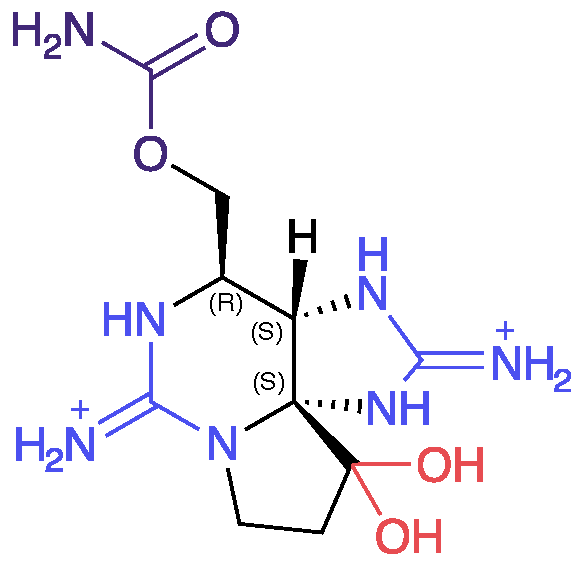
\includegraphics{stx-structure}
    \caption[Structure of STX]{Structure of STX}
    \labfig{stx-structure}
\end{marginfigure}

Having obtained a general characterization of the sunflower-type molecules and their spectroscopy, it was time to get back to the problem at hand and start looking into how they can be applied.

Let's reintroduce the molecule that motivated this whole study: saxitoxin (STX).
For the purposes of this study, the STX structure features two guanidinium moieties (which are easily susceptible to protonation), two hydroxyl, and one carbamate group as it can be seen in \reffig{stx-structure}.

The STX being doubly protonated in the figure is not an arbitrary choice.
While studying its acid-base behavior in previous work we faced a certain issue: the STX molecule has many possible protonated variations, and at the pH of real life samples, there would be a coexistence of several of them.
This was a problem, because having to apply the study to these different multiple forms in order to account for the situation would greatly increase the number of calculations.
After some thought, it was decided that the simplest way to solve this issue would be to work at a pH where only one of the protonated species would be present at a significant amount.
It was found that, at the moderate pH value of 6, the majority of the STX could be found as its doubly protonated form.
Since in real life experimental conditions attaining a pH of 6 in an hypothetical water-based sample would only imply the addition of a few drops of dilute acid, it was decided that all further studies would be carried out using such diprotonated structure.

\section{Spectroscopic study of lone STX}
The goal of this work was presented as \q{finding suitable substrate to aid in the detection of STX} from the beginning, but this desire came from a place of previous study and understanding about the spectroscopic properties of the lone STX.

This section aims to display and share the most important of these previously known facts, which are about the behavior of saxitoxin in both vibrational and electronic spectroscopy contexts.

\subsection{Vibrational spectroscopy}
As a non linear molecule with 40 atoms, STX presents a total of 114 vibrational normal modes.
Many of those modes cause changes in its polarizability, and are therefore visible in its Raman spectrum.
In this section, we pinpoint and describe a selection of the most characteristic and noticeable vibrational modes that could allow for the identification of the isolated STX.

\subsubsection{Raman spectrum}
The Raman spectrum of STX was calculated and plotted in the same way as those of the sunflowers, and displayed in both \reffig{raman-stx} and \reffig{raman-stx-zoom}.

\begin{figure}
    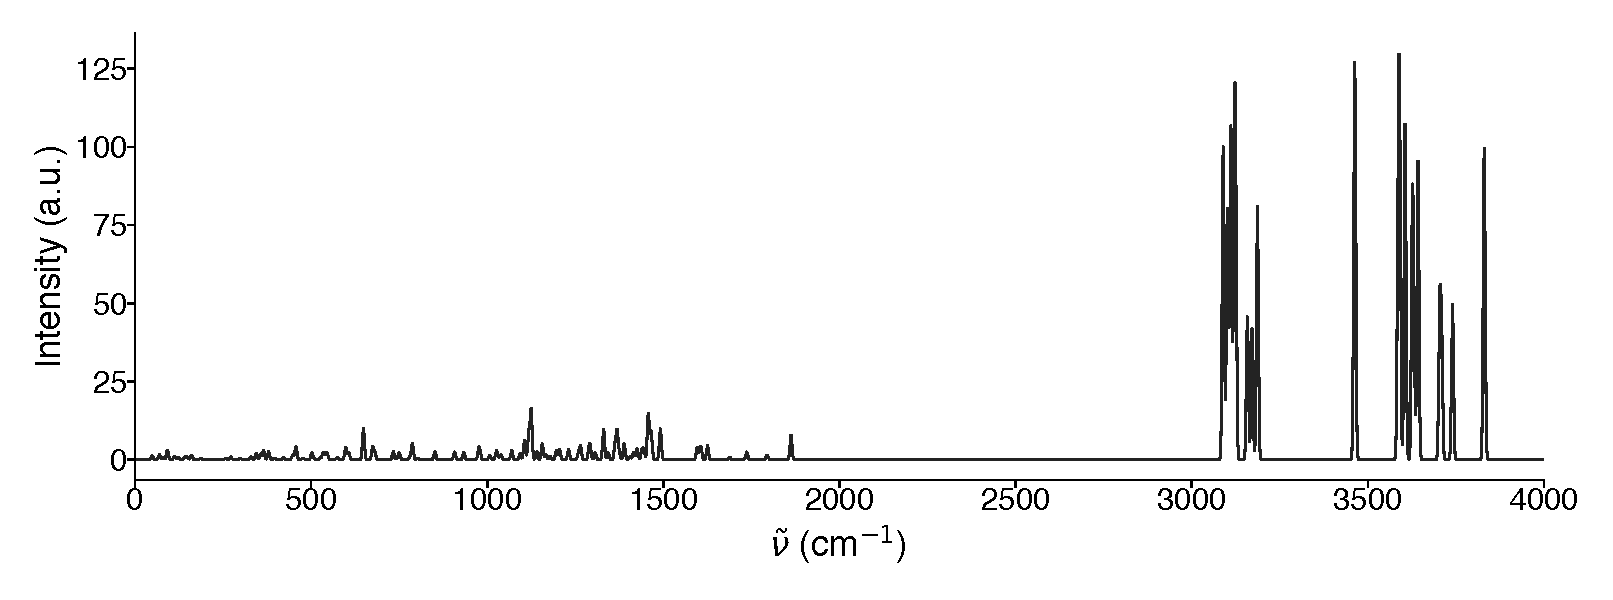
\includegraphics{raman-stx}
    \caption[Raman spectrum of lone STX]{Raman spectrum of lone STX}
    \labfig{raman-stx}
\end{figure}

\begin{figure*}
    \begin{subfigure}{8.25cm}\centering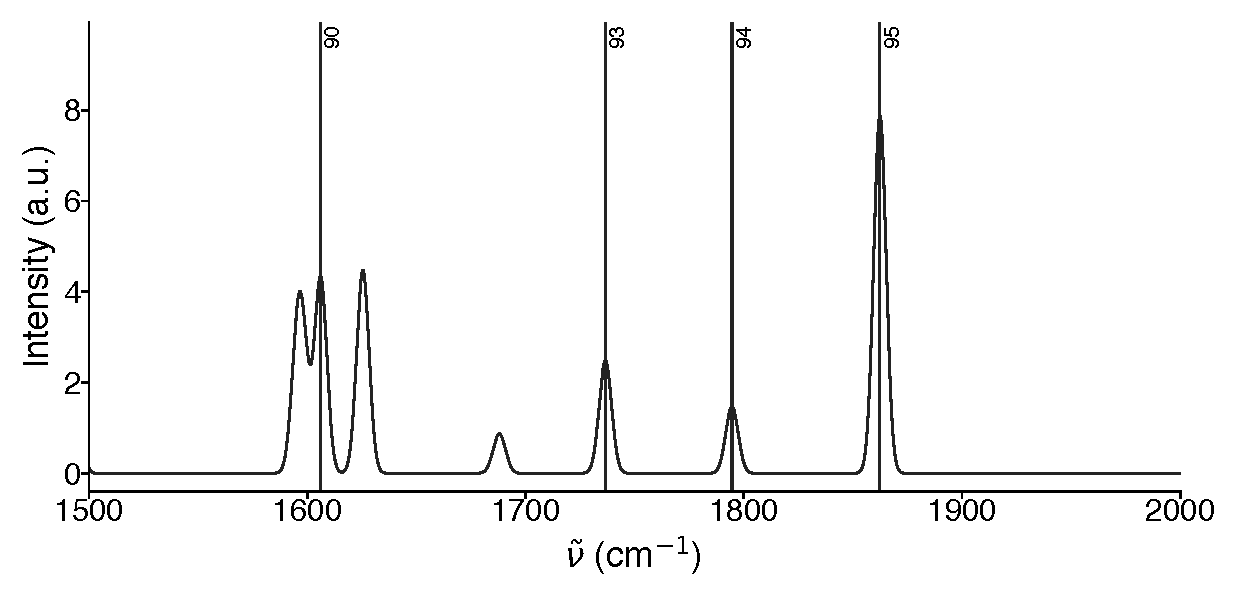
\includegraphics{raman-stx-left}\end{subfigure}%
    \begin{subfigure}{8.25cm}\centering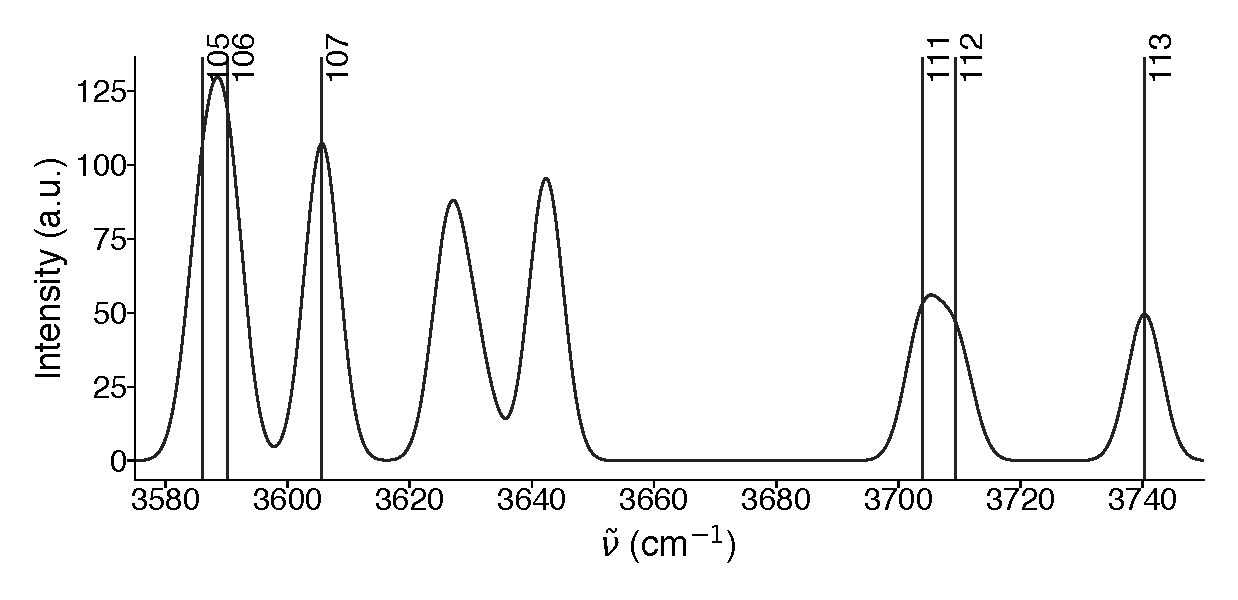
\includegraphics{raman-stx-right}\end{subfigure}
    \caption[Zoomed in Raman spectrum of lone STX]{Zoomed in Raman spectrum of lone STX with annotated vibrational modes}
    \labfig{raman-stx-zoom}
\end{figure*}

\begin{table}
    \caption[Raman modes of STX]{Selected Raman active vibrational modes for STX. Letters $\delta$ and $\nu$ are scissoring and stretching vibrations, subscripts $_\textit{s}$ and $_\textit{as}$ mean symmetric and antisymmetric; and G5, G6 and Cb are the 5 atom guanidinium moiety, the 6 atom guanidinium moiety, and the carbamate group.}
    \label{stx-modes}
    \begin{tabular}{@{}rS[table-format=4.1]r@{}}
        \toprule
        Mode & {$\tilde{\nu}$} & Description \\
        \midrule
        90 & 1606.2 & $\delta_s$ \ce{NH2} G5 \\
        91 & 1625.5 & $\delta_s$ \ce{NH2} G5 \\
        93 & 1736.6 & $\delta_s$ \ce{NH2} G6 \\
        94 & 1794.6 & $\delta_s$ \ce{NH2} G5 \\
        95 & 1862.4 & $\delta_s$ \ce{NH2}, $\nu_\textit{as}$ \ce{OCN} Cb \\
        105 & 3586.1 & $\nu_\textit{s}$ \ce{NH2} G5 \\
        106 & 3590.2 & $\nu_\textit{s}$ \ce{NH2} G6 \\
        107 & 3605.6 & $\nu_\textit{s}$ \ce{NH2} Cb \\
        111 & 3704.0 & $\nu_\textit{as}$ \ce{NH2} G5 \\
        112 & 3709.4 & $\nu_\textit{as}$ \ce{NH2} G6 \\
        113 & 3740.3 & $\nu_\textit{as}$ \ce{NH2} Cb \\
        \bottomrule
    \end{tabular}
\end{table}

These annotated modes, specified and described in \reftab{stx-modes}, were deemed as sufficient to identify the lone STX in a sample.
This is a good exercise to start identifying characteristic vibrations that could be attributed to STX.
However, it must be kept in mind that this analysis only serves as an initial approximation, as it's possible that these same vibrational modes have shifted wave numbers and/or are different when the STX gets adsorbed and forms complexes.

\subsection{Electronic spectroscopy}
\labsec{uv-stx}
STX doesn't have any special chromophore groups, and its excited states are available at the UV range of electromagnetic radiation.
Nevertheless, it's important to identify and study these transitions in order to facilitate the application of further techniques.

\subsubsection{UV-vis spectrum}
As before, using TD-DFT as implemented in Gaussian09, the first 50 electronic transitions were calculated and used to generate the UV-vis spectrum of STX, displayed in \reffig{uv-stx}.

\begin{figure}
    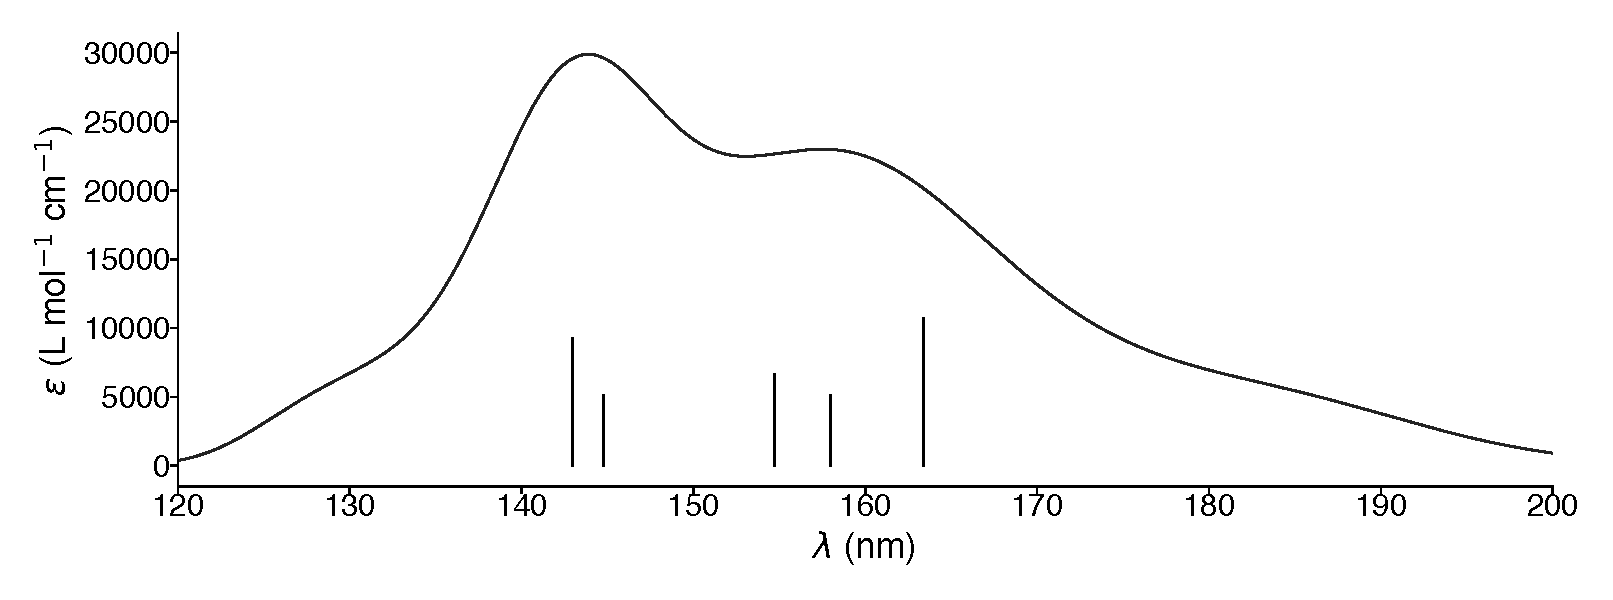
\includegraphics{uv-stx}
    \caption[UV-vis spectrum of lone STX]{UV-vis spectrum of lone STX, the 5 electronic transitions with the largest contributions have been annotated}
    \labfig{uv-stx}
\end{figure}

As it may be noted, the range of absorption (between \SI{120}{\nano\metre} and \SI{200}{\nano\metre}) is located within the UV region.
As discussed previously in \refsec{previous-work}, it's possible to induce resonance Raman effects at this wavelengths, it's just that it's expensive and impractical to use lasers that energetic in real experimental settings.
This range of UV-vis absorption need to be shifted to allow for the usage of more common incident laser wavelengths.

\section{Study of adsorption}

Having characterized the spectroscopic profile of STX, it's time to assess its interactions with the members of the sunflower family, keeping in mind the goal of determining if any of them could be a substrate suitable for its detection.
The first study that must be carried out, before any spectroscopic technique can be applied, is that of adsorption: how does STX adhere to the flowers, how stable the resulting complex is...
This is a crucial matter, as there's no point in calculating spectra for a system that isn't stable.

\subsection{Sampling and optimization}

\begin{margintable}
    \centering
    \caption[Energies of STX-S08 conformers]{Relative energies of the STX-S08 conformers, with respect to the most stable one}
    \begin{tabular}{@{}l
                       S[table-format=2.3]@{}}
        \toprule
        System ID & {Rel. E (\si{\kilo\calorie\per\mole})} \\
        \midrule
        STX-S08-1 & 0.000 \\
        STX-S08-2 & 1.337 \\
        STX-S08-9 & 7.133 \\
        STX-S08-7 & 7.504 \\
        STX-S08-6 & 9.896 \\
        STX-S08-4 & 18.554 \\
        STX-S08-3 & 20.321 \\
        STX-S08-10 & 21.734 \\
        STX-S08-5 & 22.529 \\
        STX-S08-8 & 29.715 \\
    \end{tabular}
    \labtab{stx-s08-energies}
\end{margintable}

In order to take into account the possible conformational variability, the STX was manually given an array of different relative positions and angles with respect to the surface of the flowers.
Following this idea, 10 different variations were modeled for each of the 18 STX-sunflower pairs, resulting in a total of 180 structures.
These various orientations will be referred to as \q{conformers}.
All of the conformers for each pairing were optimized at the M06-2X/def2SVP calculation level, and their final energies were compared in order to identify the most stable ones and discard the unstable.
Taking the STX-S08 system as an example, the relative energies of all of its generated conformers are displayed in \reftab{stx-s08-energies}.
As it can be seen, the most stable conformer (MSC) is STX-S08-1.
However, STX-S08-2, STX-S08-9 and STX-S08-7 are also close energy-wise.
A question arises, how can we determine which conformers are stable enough to be important, and which are not?

\begin{figure}
    \includegraphics{s08-conformers}
    \caption[Conformers of STX-S08]{Examples of conformers of the STX-S08 system, from left to right, STX-S08-1, STX-S08-9, and STX-S08-3}
    \labfig{s08-conformers}
\end{figure}

\begin{margintable}
    \centering
    \caption[Maxwell-Boltzmann populations of STX-S08]{Maxwell-Boltzmann populations of the STX-S08 conformer set, expressed as percentages}
    \begin{tabular}{@{}l
                       S[table-format=2.2]@{}}
        \toprule
        System ID & {Population (\si{\percent})} \\
        \midrule
        STX-S08-1 & 58.56 \\
        STX-S08-2 & 34.16 \\
        STX-S08-9 & 3.30 \\
        STX-S08-7 & 2.83 \\
        STX-S08-6 & 1.08 \\
        STX-S08-4 & 0.03 \\
        STX-S08-3 & 0.02 \\
        STX-S08-10 & 0.01 \\
        STX-S08-5 & 0.01 \\
        STX-S08-8 & 0.00 \\
    \end{tabular}
    \labtab{stx-s08-populations}
\end{margintable}

\subsection{Maxwell-Boltzmann statistics}
Our answer to this problem consisted in applying Maxwell-Boltzmann statistics to transform these energies into population fractions.
This concept essentially translates as the fraction of each conformer that would be present in a macroscopic sample at a certain temperature.
As modeled in \refeq{maxwell-boltzmann}, $p_i$ represents the population fraction of the conformer $i$, while $p_\textit{MSC}$ is the fraction of the MSC of that particular set of conformers.
As for the rest of the elements of the equation, $\varepsilon$ corresponds to the absolute energies of the systems, $N$ is the total number of conformers in each set (which is 10 in our case), $k$ is Boltzmann's constant, and $T$ is the temperature of the system in \si{\kelvin} (which for the purposes of this study is set at \SI{298.15}{\kelvin}).

\begin{align}
\begin{split}
    \labeq{maxwell-boltzmann}
    \frac{p_i}{p_\textit{MSC}}&=e^{\varepsilon_\textit{MSC}-\varepsilon_i/kT} \\
    \sum_{i=1}^{N}\frac{p_i}{p_\textit{MSC}}&=\frac{\sum_{i=1}^{N}p_i}{p_\textit{MSC}}=\frac{1}{p_\textit{MSC}} \\
    \frac{p_i/p_\textit{MSC}}{1/p_\textit{MSC}}&=\frac{e^{\varepsilon_\textit{MSC}-\varepsilon_i/kT}}{\sum_{i=1}^{N}\frac{p_i}{p_\textit{MSC}}}=p_i \\
\end{split}
\end{align}

Continuing with the example, the populations for STX-S08 were computed and are displayed in \reftab{stx-s08-populations}.
As an arbitrary threshold, it was decided to filter out all of the conformers with populations lower than \SI{1}{\percent}, and to just keep studying the remaining ones.
That is, all further calculations that involve the computation of weighted mean values or spectra will only take into account conformers with populations higher than that value.

\begin{table}
    \centering
    \caption[Maxwell-Boltzmann populations for all sets]{Maxwell-Boltzmann populations for the 5 most stable conformers in all sets, as percentages, with non significant conformers marked in grey}
    \begin{tabular}{@{}c
                    S[table-format=2.2]
                    S[table-format=2.2]
                    S[table-format=2.2]
                    S[table-format=2.2]
                    S[table-format=2.2]
                    S[table-format=2.2]@{}}
        \toprule
        System & {S} & {Se} & {As} & {AsN} & {P} & {PN} \\
        n of petals & {\si{\percent}} & {\si{\percent}} & {\si{\percent}} & {\si{\percent}} & {\si{\percent}} & {\si{\percent}} \\
        \midrule
        \multirow{5}{*}{08}
        & 58.56 & 79.24 & 60.96 & 81.32 & 40.79 & 65.13 \\
        & 34.16 & 15.57 & 35.22 & 15.98 & 37.48 & 29.71 \\
        & 03.30 &  1.90 &  2.19 &  2.16 & 20.53 &  4.61 \\
        &  2.84 &  1.15 &  1.38 &  \color{fd}0.25 &  \color{fd}0.44 &  \color{fd}0.24 \\
        &  1.08 &  \color{fd}0.14 &  \color{fd}0.16 &  \color{fd}0.23 &  \color{fd}0.32 &  \color{fd}0.21 \\
        \\
        \multirow{5}{*}{10}
        & 38.68 & 61.74 & 99.64 & 100.00 & 86.97 & 51.05 \\
        & 36.07 & 38.26 &  \color{fd}0.30 &   \color{fd}0.00 & 10.12 & 46.11 \\
        & 25.21 &  \color{fd}0.00 &  \color{fd}0.00 &   \color{fd}0.00 &  2.83 &  2.26 \\
        &  \color{fd}0.02 &  \color{fd}0.00 &  \color{fd}0.00 &   \color{fd}0.00 &  \color{fd}0.06 &  \color{fd}0.56 \\
        &  \color{fd}0.01 &  \color{fd}0.00 &  \color{fd}0.00 &   \color{fd}0.00 &  \color{fd}0.02 &  \color{fd}0.01 \\
        \\
        \multirow{5}{*}{12}
        & 99.99 & 58.93 & 99.75 & 97.75 & 93.29 & 93.83 \\
        &  \color{fd}0.01 & 18.98 &  \color{fd}0.10 &  2.23 &  3.26 &  5.97 \\
        &  \color{fd}0.00 & 14.52 &  \color{fd}0.08 &  \color{fd}0.01 &  2.42 &  \color{fd}0.20 \\
        &  \color{fd}0.00 &  6.03 &  \color{fd}0.04 &  \color{fd}0.00 &  \color{fd}0.74 &  \color{fd}0.00 \\
        &  \color{fd}0.00 &  1.55 &  \color{fd}0.02 &  \color{fd}0.00 &  \color{fd}0.16 &  \color{fd}0.00 \\
        \bottomrule
    \end{tabular}
    \labtab{maxwell-boltzmann-all}
\end{table}

\subsection{Basis set superposition error correction}
These optimization calculations have served as a way to estimate the populations of the conformers and to identify the most stable and relevant ones.
However, they cannot be used directly to obtain accurate values for the interaction energies due to the basis set superposition error (BSSE).
In this case, this error arises when the STX molecule is close to the sunflower and their basis functions overlap.
The part of STX basis functions that comes near the sunflower improves its part of the calculation, and vice versa.
This is a problem because in order to get the interaction energy we have to subtract the energy of the complex from the energies of the isolated molecules,\marginnote{
    \begin{equation}\labeq{interaction-energy}
        V_\textit{STX-flower} = E_\textit{STX-flower} - E_\textit{STX} - E_\textit{flower}
    \end{equation}
} but the former has a better calculation level than the latter.

To solve this problem, we used the counterpoise method.
For hypothetical molecules A and B, this technique estimates their BSSE by placing the basis functions of molecule A next to molecule B, right where molecule A would go in the optimized geometry of the complex.\sidecite{duijneveldt94,rosch03}
However, its nuclei are ommited, and just the energy of A is calculated using such an extended basis set.
The same process is applied to get the corrected energy of isolated B.
Finally, the same formula as in \refeq{interaction-energy} is applied to the new values, which results in the counterpoise corrected interaction energy.

All such energies were calculated for all of the STX-flower system conformers.
Their weighted averages using the population values of \reftab{maxwell-boltzmann-all} were computed, and are displayed in \reffig{counterpoise-energies}.

\begin{figure}
    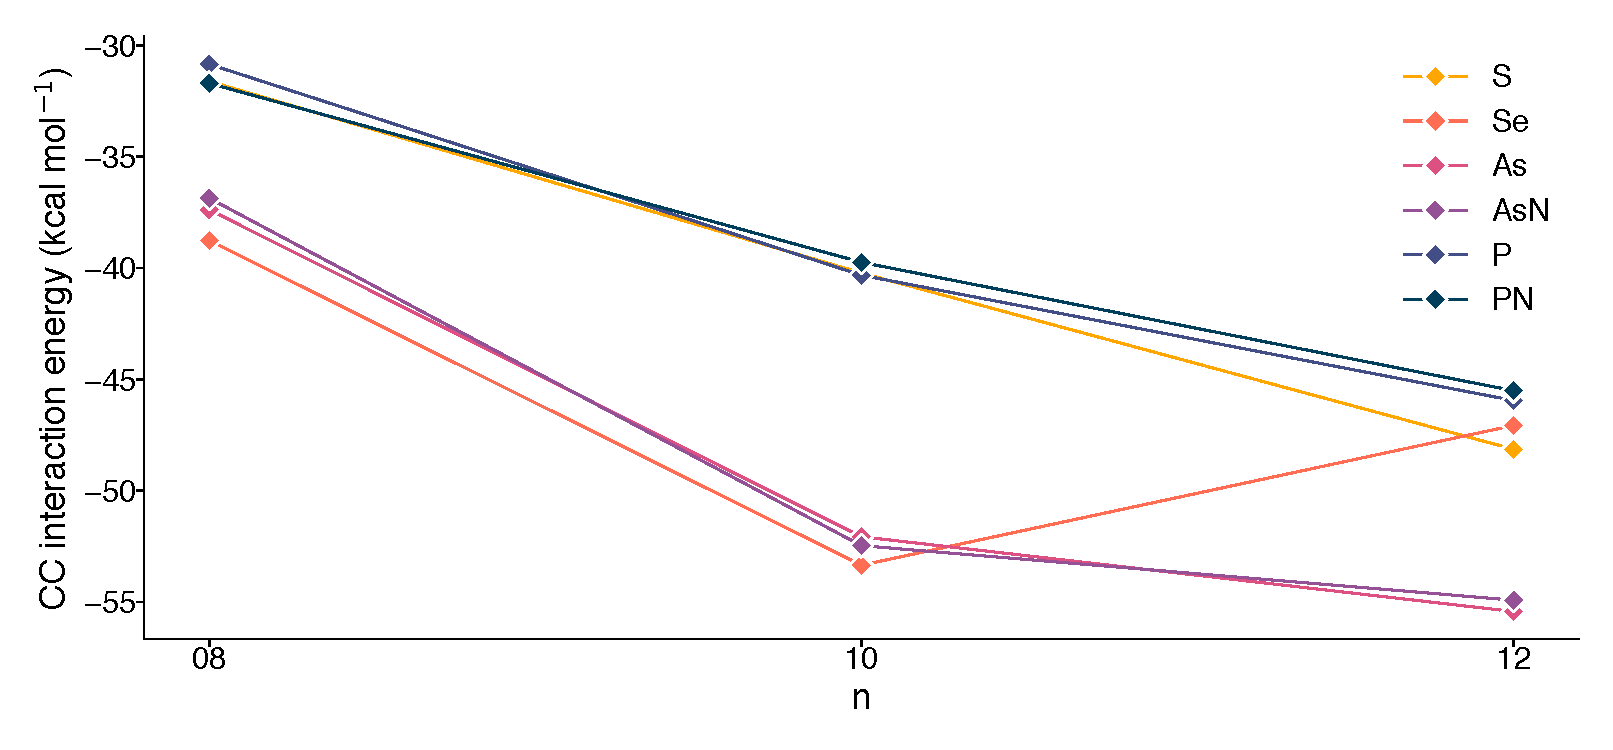
\includegraphics{counterpoise-energies}
    \caption[Counterpoise corrected interaction energies]{Counterpoise corrected interaction energies as weighted averages for all of the sets}
    \labfig{counterpoise-energies}
\end{figure}

As it can be noted, all of the systems present negative interactions energies, that is, the complex has a lower energy than the sum of the energies of its constituents.
This is a good indication that the systems are all stable and can be further studied.
All of the families (except for Se) appear to have a common tendency: the higher the amount of petals, the higher the stabilization. This could be due to the flower having a larger area and bending in a way that maximizes the interactions with the STX molecule.

\section{Study of UV-vis behavior}
\labsec{complex-uv}
One of the main points of adsorbing the STX to the flowers is the desire of increasing its range of absorption of UV-vis radiation.
It's possible that the STX-flower complex absorbs light at longer wavelengths than the isolated STX, and this could be highly beneficial to apply further detection techniques based on resonace.

\subsection{General UV-vis spectroscopy}
Electronic spectra were calculated as described in \refsec{electronic-transition-study} and \refsec{spectra-envelope-calculation} for the most stable conformers of all of the STX-flower complexes.

First, they were plotted together with the UV-vis spectrum of STX and of their corresponding isolated flower.
The individual transitions with significant weights were also plotted as straight vertical lines.
This allowed us to compare the absorption ranges of the complex versus those of the isolated STX and flowers, and to judge if the shifting effect is good enough.

As an example of this, the UV-vis spectra of STX, S08 and S08-STX are displayed in \reffig{uv-s08}.

\begin{figure}
    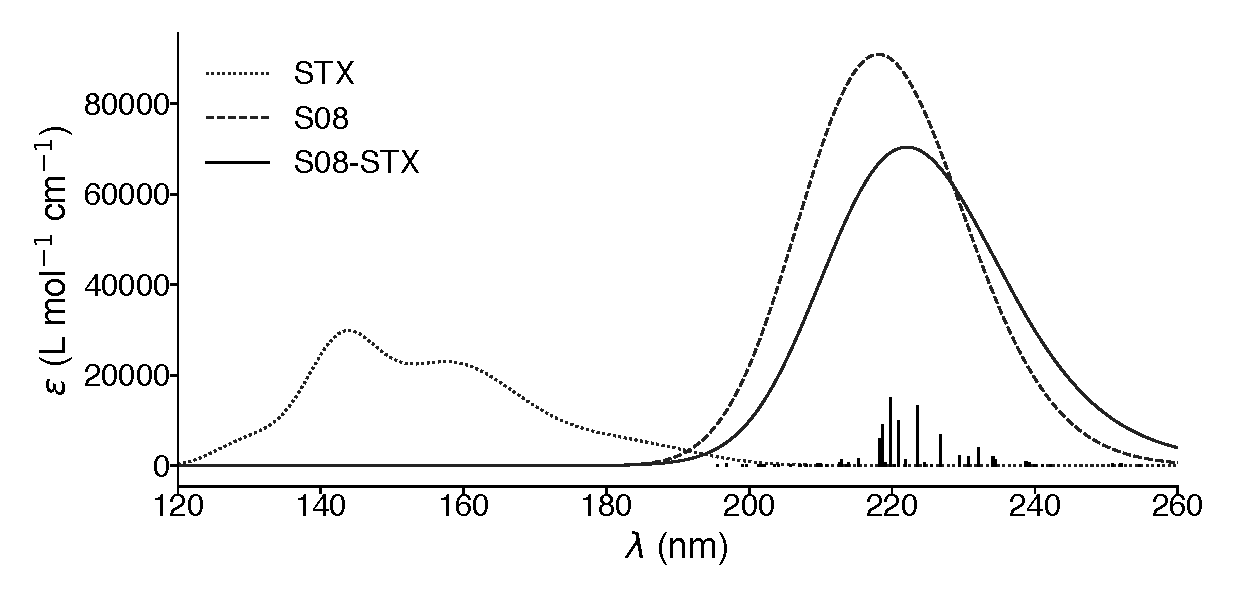
\includegraphics{uv-s08}
    \caption[UV-vis spectrum of S08-STX]{UV-vis spectra of S08-STX and its components}
    \labfig{uv-s08}
\end{figure}

As it may be noted, the spectra of the complex has almost the same absorption range as that of the isolated S08, and in any case, it's definitely shifted towards longer wavelengths in contrast with that of STX.
This effect was the same for all of the STX-flower complexes, and the full list of compared UV-vis spectra can be found in \refsec{ap:uv-vis-flowers}.

After this, the UV-vis absorption spectra of all of the complexes were plotted together in order to visually compare just their absorption ranges. This plot is displayed in \reffig{complex-uv}, where the main heteroatoms of the flowers and their number of petals are distinguished using different colors and linestyles, respectively.

\begin{figure*}
    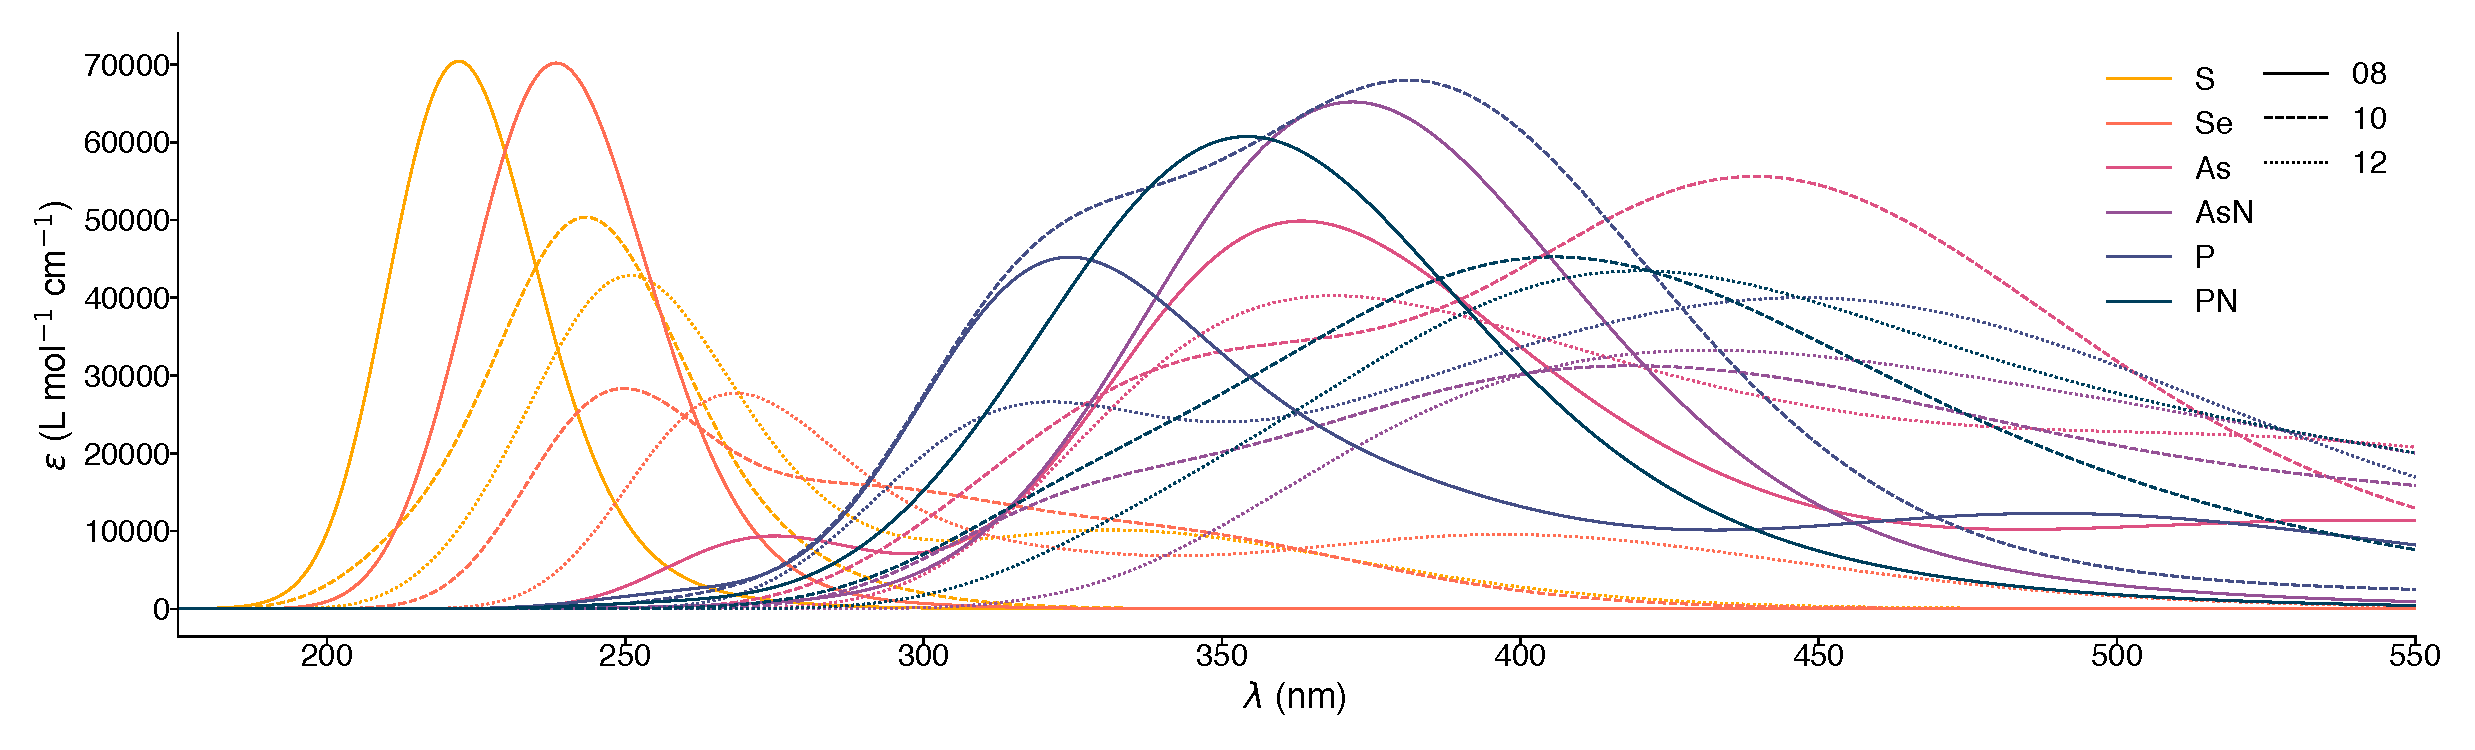
\includegraphics{complex-uv}
    \caption[UV-vis absorption spectra of all complexes]{UV-vis absorption spectra of all STX-flower complexes}
    \labfig{complex-uv}
\end{figure*}

Since this work aims to propose realistic detection techniques, it's important that the systems are actually detectable and identifiable in a real setting.
With this purpose in mind, and keeping into account the usual wavelengths of commercially available lasers for Raman,\sidenote{Which is between \fix{\SI{300}{\nano\metre} and \SI{800}{\nano\metre}}} all of the complexes with absorption ranges starting below \SI{250}{\nano\metre} were filtered out.
From the remaining ones, a select few were hand-picked according to the upper limit of their ranges and to their specific individual electronic transitions.
This left us with 8 systems out of the starting 18, which was deemed as a sufficient amount to continue with the last part of the study.

\begin{margintable}
    \centering
    \caption[UV absorption range of selected complexes]{UV absorption range of selected complexes}
    \begin{tabular}{@{}rc@{}}
        \toprule
        System & $\lambda$ (\si{\nano\metre}) \\
        \midrule
        As10 & 300-600 \\
        As12 & 300-900 \\
        AsN08 & 300-450 \\
        AsN10 & 300-650 \\
        AsN12 & 350-850 \\
        P12 & 300-700 \\
        PN10 & 300-550 \\
        PN12 & 325-625 \\
    \end{tabular}
    \labtab{uv-ranges}
\end{margintable}

The UV absorption range for those remaining complexes was also displayed on \reftab{uv-ranges} for convenience.
\blindtext

\section{Resonance Raman}
At last, it was time to apply the previous parts of the study and test the performance of the selected sunflowers.
As seen in \refsec{complex-uv}, all of these complexes have absorption ranges that could be useful in real life, and all of them should be able to be subject the resonance Raman phenomenon.
The main point of this section is generating actual amplified Raman spectra, identifying the lasers that would produce the best amplifications, and being able to select a flower that makes the identification of STX easier.

\subsection{Generation and comparison of spectra}
\labsec{heatmaps}
RR spectra were generated for each of the STX-flower systems by using incident laser wavelengths in their particular ranges of absorption.
Specifically, the whole of their absorption interval was covered by selecting wavelengths with a step of \SI{3}{\nano\metre}.\sidenote{So in the case of As10, for example, the Resonance raman calculations were performed with lasers of \num{300}, \num{303}, \num{306}... all up until \SI{600}{\nano\metre}}

The RR calculations from this step amounted to a total of 2858, where the amplification, position and relevance of each vibrational mode\sidenote{\num{186}, \num{204} or \num{222} depending on the size of the flower} had to be evaluated.
For this purpose, the two following metrics were developed.

\subsubsection{Individual molecule contribution to a complex vibrational mode}
The first of these evaluations was differentiating which vibrational normal modes involve the vibration of the flower, which modes involve the vibration of the STX, and which modes are mixed.
As introduced in \refsec{intmodes-methods}, this was done by analyzing the displacements of the vibrations translated into redundant internal coordinates.
To understand how this is done, we will use the As12-STX system as an example.
The standard Gaussian09 output describes normal modes as cartesian displacements of normal coordinates, indicating vectors for each atom.
For instance, the beginning of the output of vibrational normal mode number 42 looks like this:

\begin{lstlisting}[label=normal-mode-output, style=kaolstplain]
                    42
                     A
Frequencies --    229.2846
Red. masses --     36.2305
Frc consts  --      1.1222
IR Inten    --      3.9161
Atom  AN      X      Y      Z
   1  33    -0.15  -0.08   0.01
   2  33    -0.03  -0.04  -0.04
   3   6     0.13   0.06   0.06
   4   6     0.06   0.05   0.01
   5  33     0.10  -0.01  -0.03
               ...
\end{lstlisting}

This contains all of the necessary information to study the movements of the atoms and understand the vibrations of the mode, but it's difficult to interpret.
By specifying the keyword \code{intmodes} in the frequency calculation, this output gets translated into the much more readable redundant internal coordinates notation.
This is As12-STX's mode number 42 in this new format.

\begin{lstlisting}[label=intmodes-output, style=kaolstplain]
              ----------------------------
              ! Normal Mode    42        !
--------------                            --------------
! Name  Definition       Value     Relative Weight (%) !
--------------------------------------------------------
! R1    R(1,34)         -0.0693             0.4        !
! R9    R(4,63)         -0.067              0.4        !
! R15   R(8,9)           0.1332             0.8        !
! A4    A(2,3,30)       -0.0755             0.4        !
! A19   A(10,7,63)       0.0567             0.3        !
! A21   A(5,9,8)         0.1548             0.9        !
! D1    D(36,1,34,24)    0.0965             0.5        !
! D3    D(34,1,36,27)    0.1767             1.0        !
! D5    D(6,2,3,4)      -0.0882             0.5        !
                          ...
\end{lstlisting}

\begin{margintable}
    \centering
    \caption[Classification of individual vibrations]{Classification of the individual vibrations of normal mode 42 for As12-STX (atoms of the flower and the STX are marked in blue and red, respectively)}
    \begin{tabular}{@{}ll@{}}
        \toprule
        Vib. def. &  Category \\
        \midrule
        R(\stx{1},\stx{34})                     & STX \\
        R(\stx{4},\flower{63})                  & Mixed \\
        R(\stx{8},\stx{9})                      & STX \\
        A(\stx{2},\stx{3},\stx{30})             & STX \\
        A(\stx{10},\stx{7},\flower{63})         & Mixed \\
        A(\stx{5},\stx{9},\stx{8})              & STX \\
        D(\stx{36},\stx{1},\stx{34},\stx{24})   & STX \\
        D(\stx{34},\stx{1},\stx{36},\stx{27})   & STX \\
        D(\stx{6},\stx{2},\stx{3},\stx{4})      & STX \\
    \end{tabular}
    \labtab{intmodes-classification}
\end{margintable}

Here the displacements are expressed as bond length extensions between two atoms (R), angle openings and closings between three (A), and dihedral angle torsions between four (D).
Their magnitude is expressed as a single positive or negative value, whose absolute value is then weighted and displayed as the Relative Weight as a percent.
By differentiating whether the atoms involved in a certain vibrational motion belong to the As12 flower or to the STX, said vibration can be classified as an exclusive flower vibration, as an exclusive STX vibration, or as a mixed one.
Such classification, illustrated in \reftab{intmodes-classification}, can be easily automated using a script.

By adding up the relative weights of the vibrations in each category, we can find out which of the elements of the STX-flower complex dominate a particular mode.
In this case, mode 42 has a \SI{92.54}{\percent} contribution from the STX, a \SI{0.00}{\percent} contribution from the flower, and a \SI{7.45}{\percent} contribution from mixed vibrations.

From a practical point of view, the fact that it's composed almost exclusively of isolated STX vibrations makes this a good choice of vibrational mode to look for in a RR spectra of this complex.
In contrast to other mixed or flower-exclusive vibrational modes, a mode like this is a clear sign of the presence of the STX.

\subsubsection{Resonance Raman enhancement factor}
Even if a mode is exclusive to our molecule of interest, it needs to have a sufficient intensity in the final spectrum: otherwise it cannot be detected and cannot be of any use in the identification.
In the context of RR, this means that it has to benefit from a certain level of amplification during resonance experiments.

To evaluate this for all of the tested laser wavelengths, the enhancement factor (EF) metric was designed and applied.
The EF for a certain vibrational mode $i$ and laser wavelength $\lambda$ is defined in \refeq{enhancement-factor}.

\begin{equation}
    \labeq{enhancement-factor}
    EF_{i,\lambda} = \log_{10}\left(\frac{I_{i,\lambda}}{I_{i,\textit{SL}}}\right)
\end{equation}

In this equation, $I_{i,\lambda}$ corresponds to the Raman activity of the mode $i$ in the amplified spectrum, and $I_{i,\textit{SL}}$ is the activity of the same mode in a regular Raman prediction.
Using a logarithmic scale makes easier to visualize the very high amplifications that arise with this technique, which in the case of this work, have reached values near \num{10e10} times than the standard Raman.

Similarly as before, this calculation is easy to automate and can serve as a way to filter out wavelengths that don't generate sufficient amplification, or discard modes that aren't sufficiently amplified.

\subsubsection{Combined resonance graphs}
In order to make use of the two newly defined metrics, an output file processing pipeline was designed.
Large amounts of data from the internal mode decompositions, standard Raman spectra and many amplified RR spectra were processed, combined and analyzed using Python scripts.

This information was filtered and displayed in the following manner:
First, Gaussian envelopes for all of the RR spectra as well as the standard Raman spectrum were calculated.
These envelopes were equivalent to those used in previous Raman spectra: \num{10000} points divided across the most relevant range for each system.
Then, each of the points in the amplified RR curves was converted into EF values using \refeq{enhancement-factor}.
These were plotted as a colored grid: all of the RR wavelengths on the vertical axis, and the \num{10000} calculated wave number values on the horizontal axis.
The squares of the grid, therefore, were colored according to the calculated EF values.

This resulted in quite colorful graphs where the brightest horizontal lines correspond to the laser wavelengths that generate larger amplifications, and bright vertical areas correspond to highly amplified vibrational modes.

Then, in order to make full use of the metrics, these graphs were annotated using a special procedure.
In regard to the vibrational modes, two thresholds were set: a maximum percent of flower contribution, and a minimum percent of STX contribution.
This ensured that the displayed modes were relevant.
As for the laser wavelengths, only the ones that produced amplifications above a certain threshold value for the EF of the previously selected vibrational modes were displayed.

It should be noted that the values of these metrics varied very significantly between the different systems.
Therefore, setting common thresholds for all of them was unpractical: the values that worked for a certain complex were too strict for others.
For this reason, the thresholds were set individually for each of the systems in a such a way that only the top 5, 6 or 7 lasers and the best 5, 6 or 7 vibrational modes were selected and labeled.
The cutoff values for these top results, therefore, were annotated in each of the graphs.

Applying this method to the running example of AsN12-STX, then, resulted in \reffig{comb-asn12}

\begin{figure}
    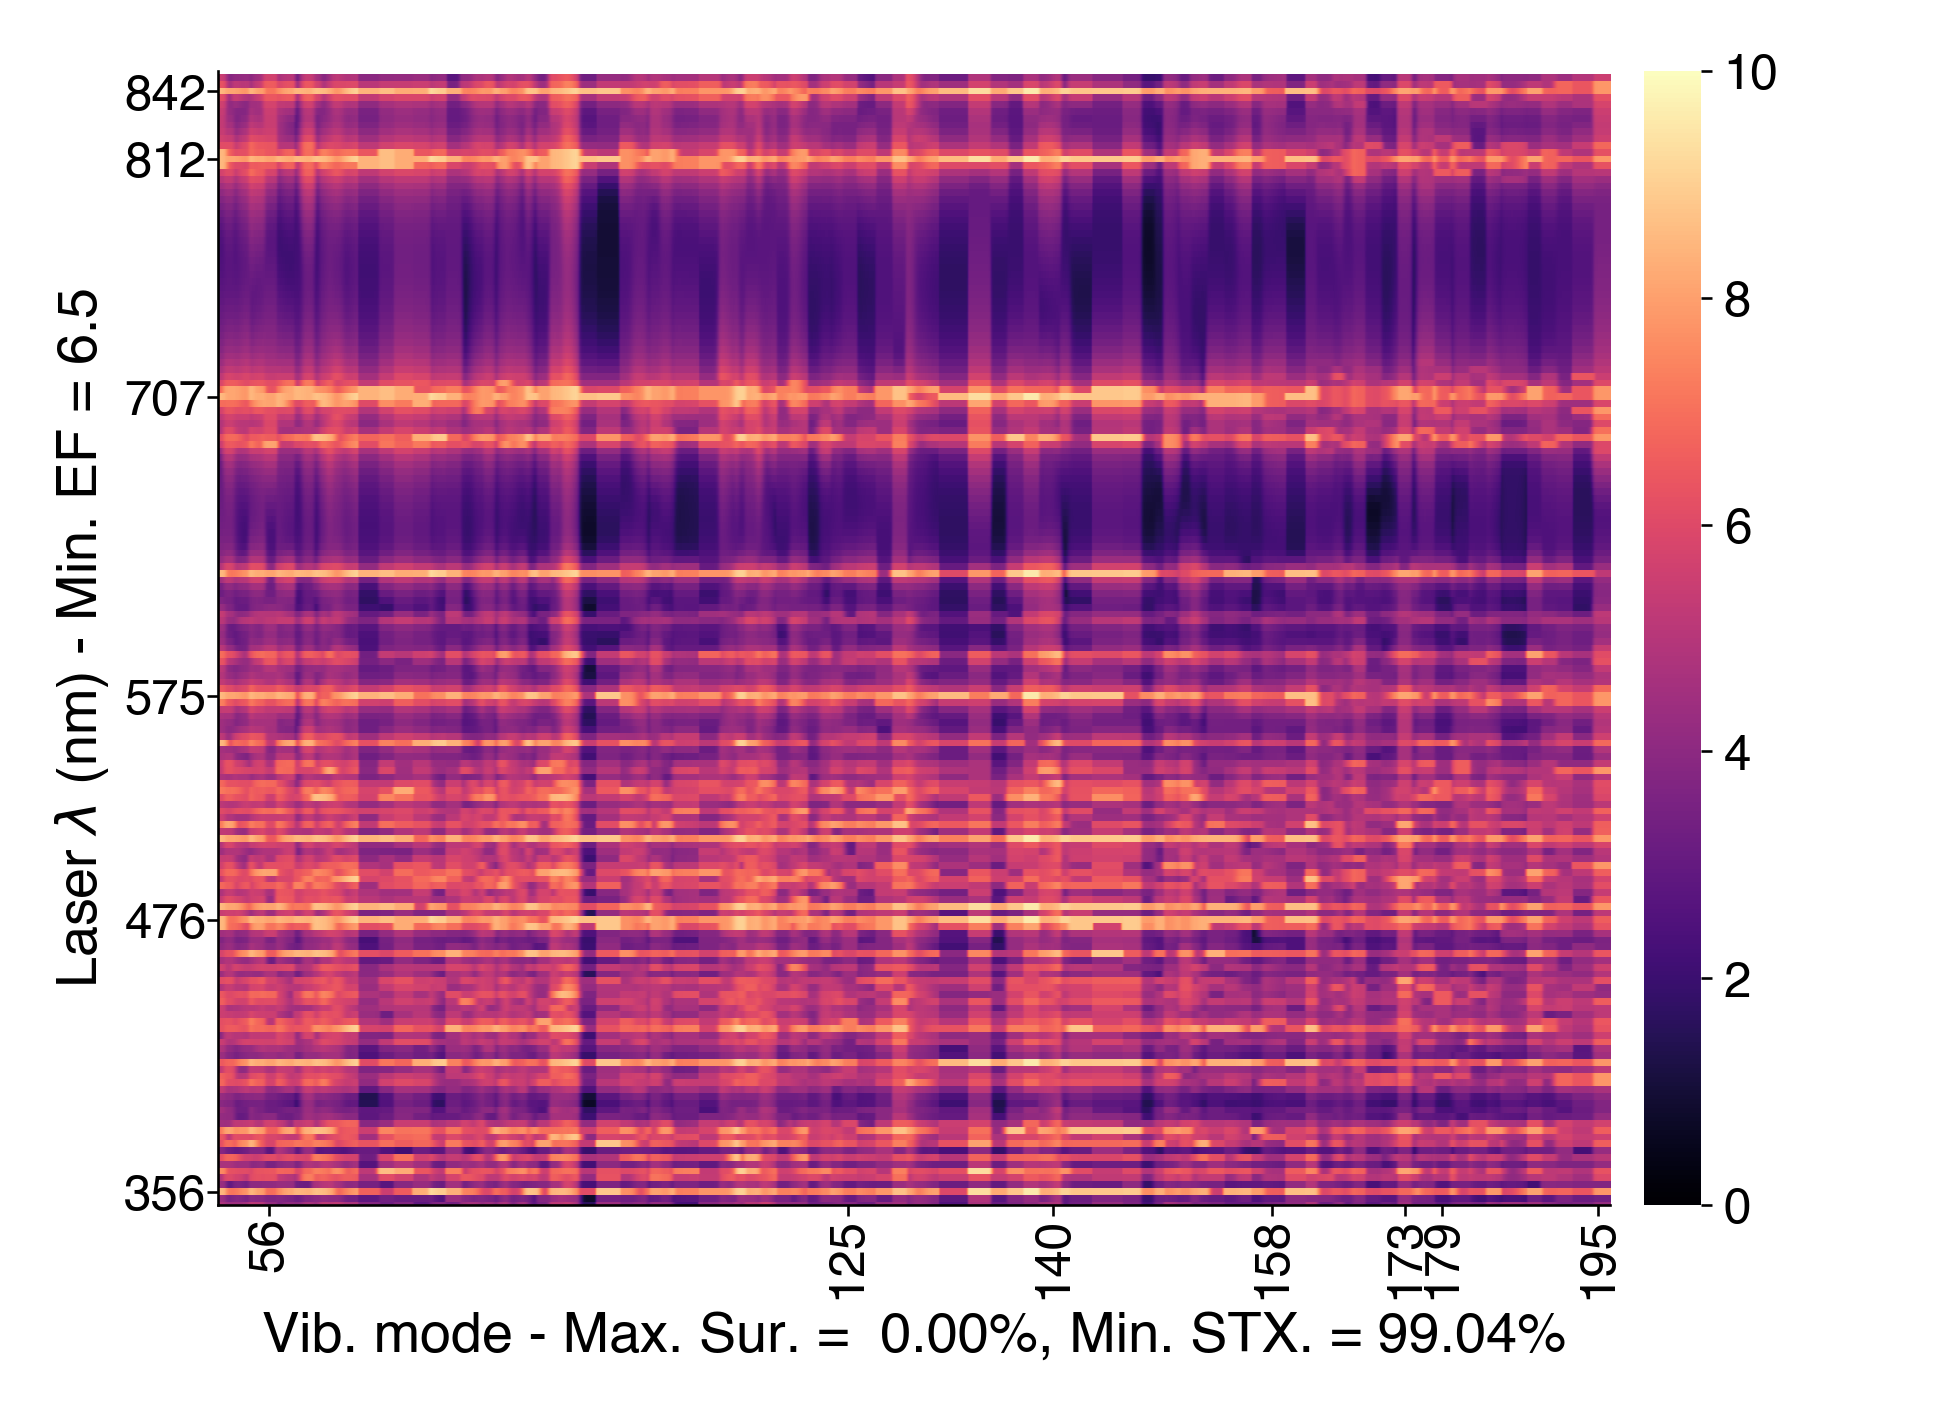
\includegraphics{comb-asn12}
    \caption[Combined resonance graph for AsN12-STX]{Combined resonance graph for AsN12-STX}
    \labfig{comb-asn12}
\end{figure}

\begin{margintable}
    \centering
    \caption[Electronic transitions of AsN12-STX]{Major electronic transitions of AsN12-STX}
    \begin{tabular}{@{}S[table-format=3.1]
                       S[table-format=1.4]@{}}
        \toprule
        {$\lambda$ (\si{\nano\metre})} & {f (a.u.)} \\
        \midrule
        366.8 & 0.0746 \\
        375.0 & 0.0986 \\
        407.7 & 0.1021 \\
        548.3 & 0.1972 \\
        599.8 & 0.0117 \\
        638.6 & 0.0052 \\
        794.27 & 0.0089 \\
    \end{tabular}
    \labtab{asn12-transitions}
\end{margintable}

As it can be observed, the laser wavelengths with the highest amplifications can be clearly distinguished at sight as bright yellow horizontal lines.
Comparing these wavelengths to those of the major electronic transitions found in the UV-vis spectra, most of them are found matching.
The UV-vis spectrum of ANs12-STX and some of its most relevant transitions have been included in \reffig{uv-asn12} and \reftab{asn12-transitions}.
This confirms that the amplification effect is related to the molecule reaching excited electronic states, supporting the theory behind resonance Raman.
While many of the bright horizontal lines of the graph don't have a label, they have great enhancement factors nonetheless; they just weren't marked because the amplification of the selected modes were not particularly high in comparison with the amplification of other less relevant ones.

\begin{figure}
    \includegraphics{uv-asn12}
    \caption[UV-vis spectrum of AsN12-STX]{UV-vis spectrum of AsN12-STX, with its 50 major transitions plotted as vertical lines}
    \labfig{uv-asn12}
\end{figure}

The main reasonings behind this interpretation are valid for the rest of the combined EF graphs, which can be found in \refsec{ap:combined-ef}, and its possible to quickly visually identify the best laser wavelengths and vibrational modes for all of them.
However, it was also possible to see that one of them presented better properties than others.

\begin{figure}
    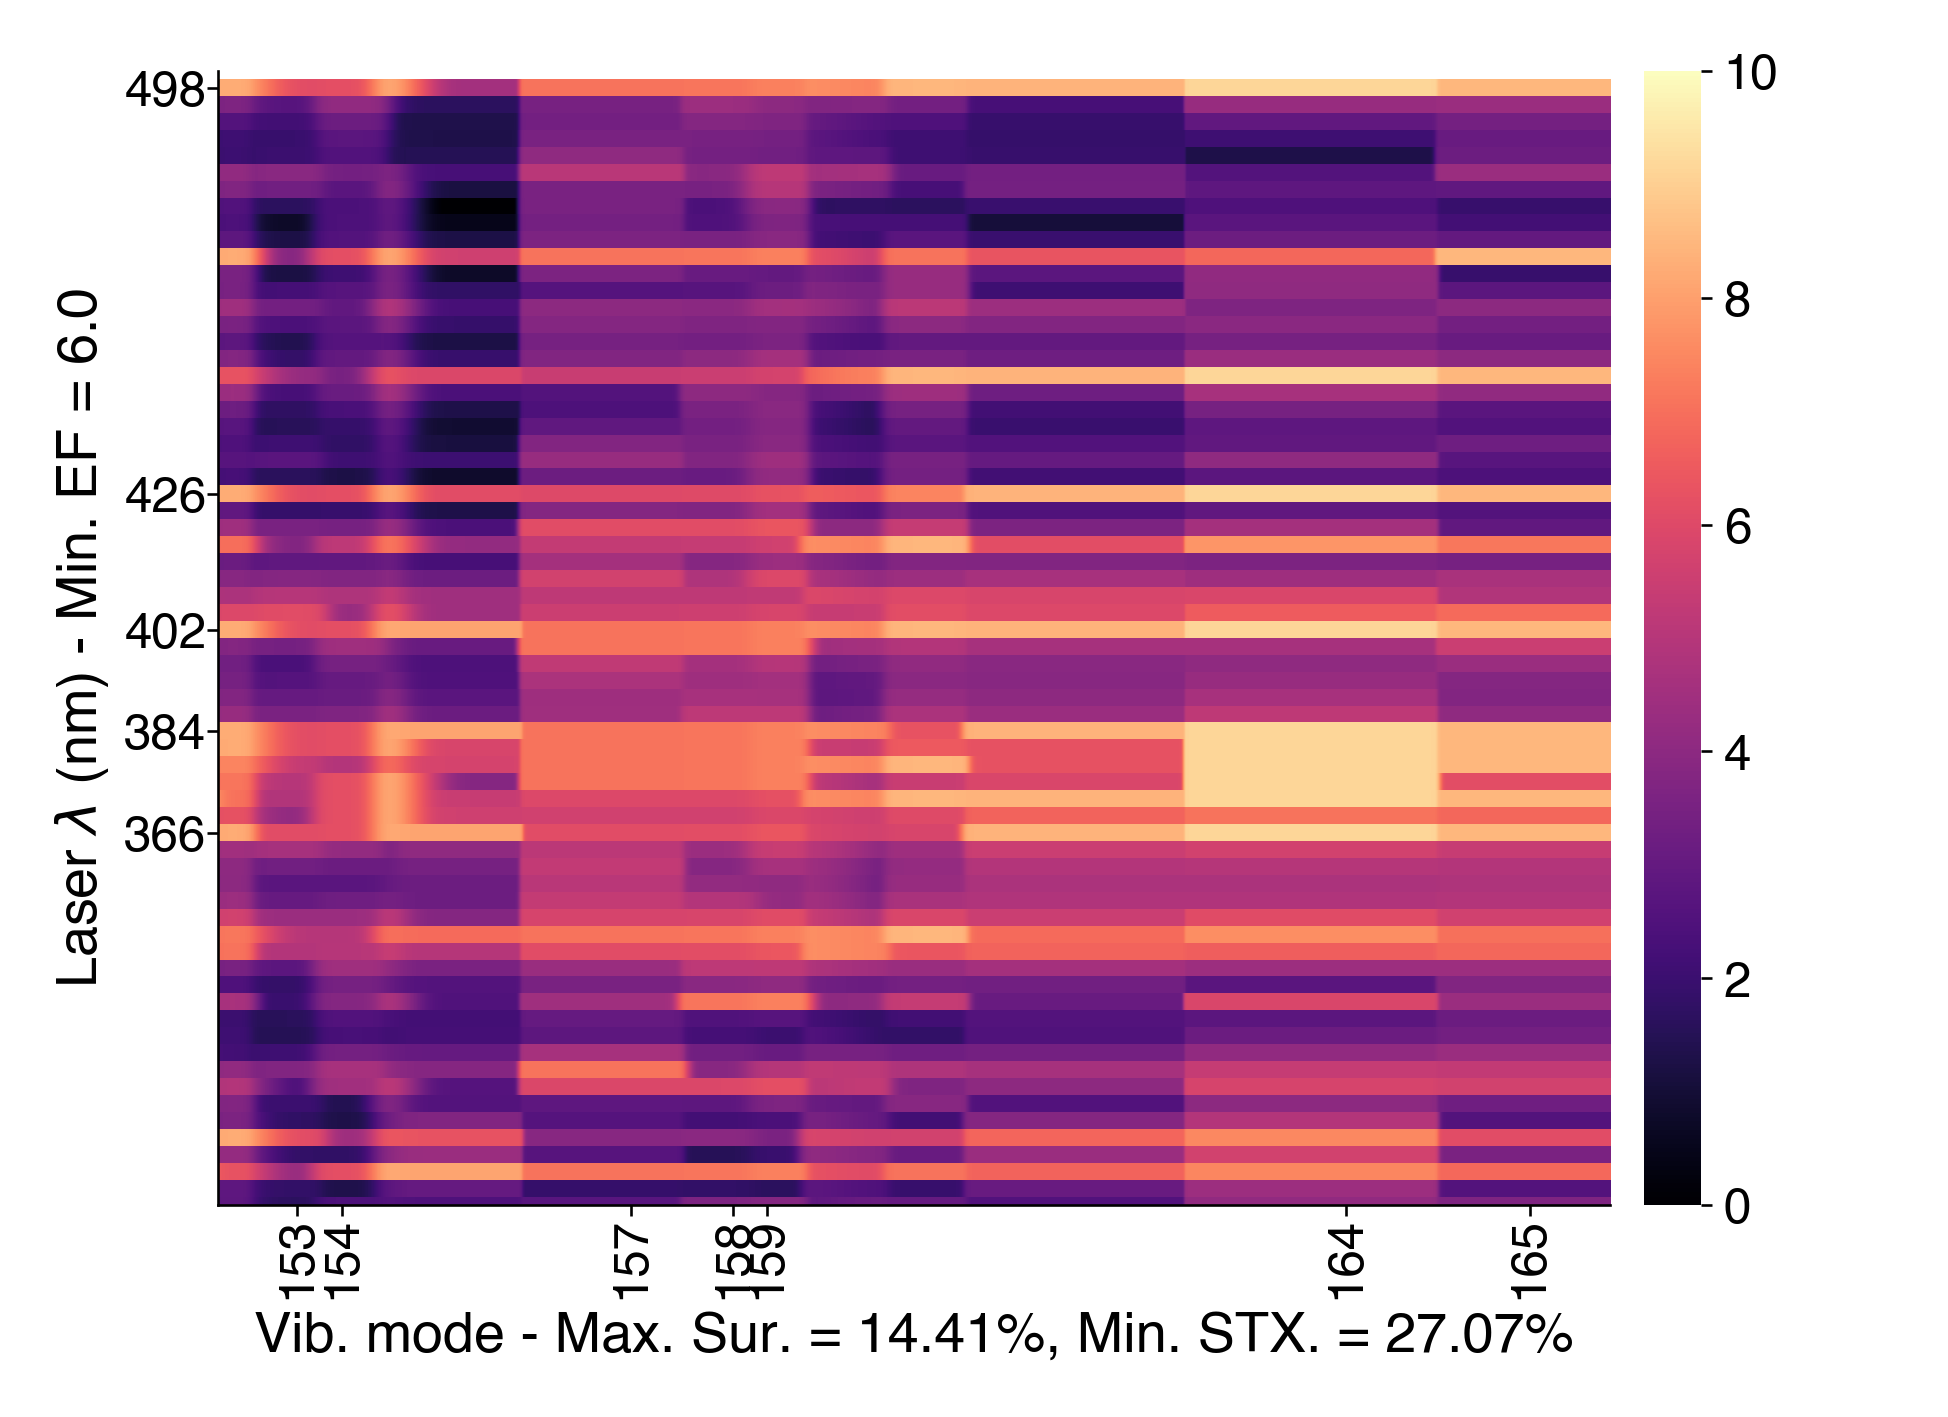
\includegraphics{comb-asn08}
    \caption[Combined resonance graph for AsN08-STX]{Combined resonance graph for AsN08-STX}
    \labfig{comb-asn08}
\end{figure}

Let's take the AsN08-STX system.
Its combined graph is similar to that of AsN12-STX in the sense that it's easy to interpret and it has a similar number of labels.
However, looking at the cutoff values, it can be observed that the ones for AsN08-STX are lower.
For example, the cutoff value for the EF in the AsN08-STX system is \num{6.0}, while in the AsN12-STX system it's \num{6.5}.
From a vibrational mode composition point of view, AsN08-STX's most pure vibrations were only guaranteed to have more than \SI{27.07}{\percent} STX contribution; while for AsN12-STX the labeled modes had over \SI{99.04}{\percent}.
It appeared that the flowers with a higher number of petals allowed for greater amplifications and more pure vibrational modes.
The exception to this tendency was PN12-STX, which had vibrational modes much less pure than the rest of 12-petal systems.

\subsection{Final selection}
While the previous method serves as a convenient way to visualize the best amplifications, it's true that it deviates a little from the usual representations of Raman data.
This final section aims to tie this insight together, and to display it in a more standard way in order to facilitate the comparison and selection of a definitive combination of flower, laser wavelength, and set of vibrational modes.

For this reason, a complementary way of plotting amplified Raman spectra was designed: drawing the amplified RR spectra of all of the previously selected laser wavelengths vertically sorted in a single plot.
The graphs in this section don't include any units of intensity: the reason for choosing these wavelengths, precisely, was that they had high enough amplifications.

\begin{figure*}[h]
    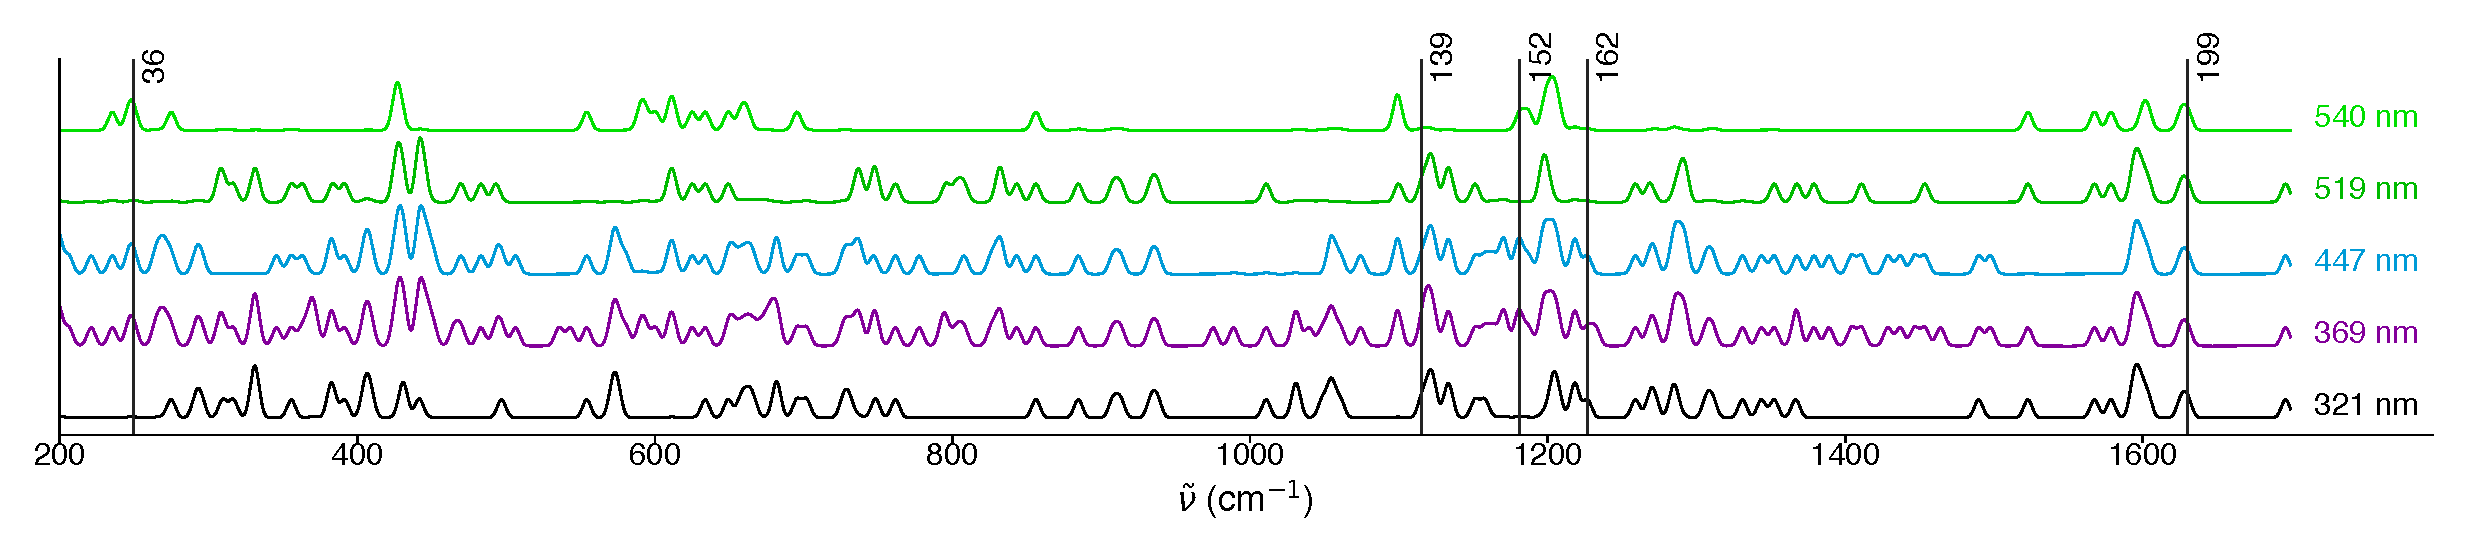
\includegraphics{unfolded-p12}
    \caption[short]{long}
    \labfig{body:unfolded-p12}
\end{figure*}

Taking the P12-STX system as an example due to its clarity, the RR spectra for its selected wavelengths were plotted and displayed in \reffig{body:unfolded-asn12}.
Using this type of graph, one can easily compare which modes have the best amplifications at each of the considered wavelengths.
In this case, it can be observed that mode 36 is only visible at \SI{369}{\nano\metre}, \SI{447}{\nano\metre} and \SI{540}{\nano\metre}.
Mode 139 can be detected with all of the laser wavelengths except for \SI{540}{\nano\metre}.
However, mode 162 is only active at \SI{321}{\nano\metre}, \SI{369}{\nano\metre} and \SI{447}{\nano\metre}.
Following this kind of logic, it's possible to select the wavelength that maximizes the number of relevant vibrational modes that are visible.
This set of vibrational modes and this laser wavelength, then, would be the ones that could be used in an analytical setting to detect and quantify the presence of STX in a sample.
In the case of P12-STX, then, the chosen wavelengths could be \SI{369}{\nano\meter} or \SI{447}{\nano\meter}, given that all of the chosen vibrational modes (\num{36}, \num{139}, \num{152}, \num{162} and \num{199}) are visible in their amplified spectra.

All of the RR spectra for the rest of the flower-STX systems can be found in \refsec{ap:rr} along the corresponding commentary.

As a way of clearly displaying these final results and selection, a last way of plotting the Raman data of a single incident laser wavelength was devised.
This one, in addition to displaying the main Raman spectrum and the labels of the main vibrational modes, also included a representation of its numerically calculated derivative.
This type of representation was applied to the P12-STX system using the previously chosen \SI{447}{\nano\meter} incident laser wavelength, and displayed in \reffig{body:final-p12}

\begin{figure*}[h]
    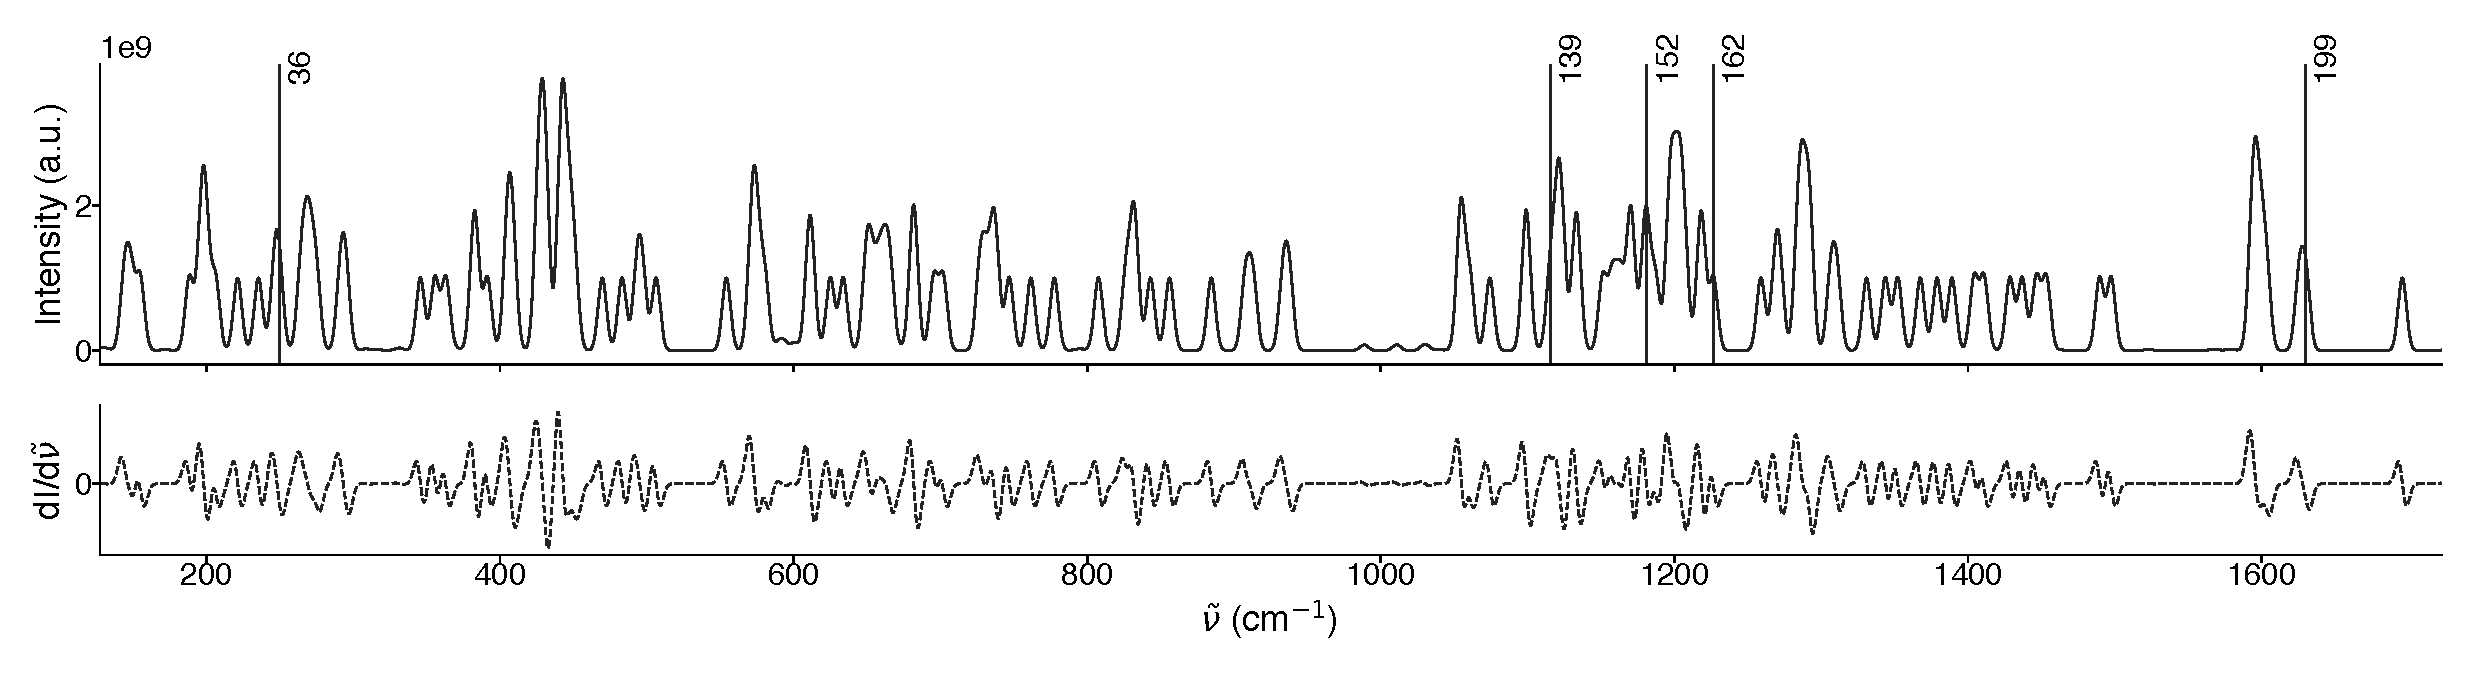
\includegraphics{final-p12}
    \caption[short]{long}
    \labfig{body:final-p12}
\end{figure*}

As it can be observed, the selected vibrational modes are clearly distinguishable, and the shape of the Raman peaks is more clear as there's only one line.
At the chosen incident laser wavelength, they are all highly amplified (in the order of \num{1e9} a.u., with EF values higher than \num{5.4}).
The addition of the derivative makes it easier to locate the peaks and evaluate their cleanliness.


\section{Conclusions}

Again, listing the most important points of this chapter as a form of conclusion:

\begin{itemize}
    \item STX+2 was previously found to be the only protonated species present at the gentle pH of 6 (in contrast with higher pH values, where multiple protonated species coexisted), so the whole study was carried out using this structure
    \item STX's vibrational spectroscopic profile was described by studying its Raman spectrum and selecting its key vibrations
    \item The electronic spectroscopy of STX was studied by generating its UV-vis spectrum
    \item STX's UV-vis absorption range, from \SI{120}{\nano\metre} to \SI{200}{\nano\metre}, was considered too low in the spectrum of light to apply resonance Raman amplification in a real life setting. This was the main motivation behind the application of sunflowers as substrates
    \item It was found that there were stable conformations for all of the flower-STX complexes. The importance of these conformers was evaluated using Maxwell-Boltzmann statistics
    \item Their corrected interaction energy was calculated using the Counterpoise method, and it was found that larger flowers tended to form more stable complexes
    \item The UV-vis spectra for all of the flower-TX complexes were generated and compared to those of the isolated flowers and STX. It was observed that in all cases the absorption ranges were greatly shifted towards larger wavelengths, but only 8 of the 18 flowers were selected to continue with the study due to their better properties
    \item A method to quantitatively evaluate the contributions of each of the molecules of a complex to a its compound vibrational modes was developed. It was applied to the flower-STX complexes in order to select the modes with the highest STX contributions
    \item The enhancement factor, a metric to evaluate the amplifications caused by a laser of a certain wavelength in a RR setting, was defined. It was applied to the flower-STX complexes to select the best lasers based on how much they amplified the intensity of the previously chosen vibrational modes
    \item A final selection of normal vibrational modes and laser wavelengths was done for each of the 8 flower-STX complexes, and it was displayed in two different forms
\end{itemize}

In general, the outcome of this chapter was considered a success.
Many of the proposed sunflowers were considered appropriate for the STX molecule resulting in great amplifications of their key modes, and in the end, realistic combinations of vibrations and lasers were selected for each of them.
